\documentclass[a4paper,11pt]{article}
\usepackage[utf8]{inputenc}
\usepackage[english]{babel} % Adds processing for some simple special characters.

% Packages for better page formatting and nice footnotes. %

\usepackage{fancyhdr} % Headers.
\usepackage{multicol} % Columns.
\usepackage[margin=0.75in]{geometry} % Margins.

\pagestyle{fancy}
\fancyhf{} % What does this do?
\lhead{Alexander S. Wheaton}
\rhead{\thedate}
\cfoot{Page \thepage}

\renewcommand{\thefootnote}{\fnsymbol{footnote}}

% Title and author for title page. %

\title{Deep Stacking of AGN Hypervariables}
\author{
    Alexander S. Wheaton\\
    School of Physics and Astronomy\\
    The University of Edinburgh\\
    s1572046@ed.ac.uk\break
}

% Utilities for fine-grained control over image insertion. %

\usepackage{graphicx} % Insert images.
\usepackage{float} % Images float in document environment.
\usepackage{wrapfig} % Image/tables in multicols with \wrapfigure or \wraptable.
\usepackage{caption} % Captions for single images.
\usepackage{subcaption} % Captions for simultaneous images.
\graphicspath{ {./img/} }

% Not sure what this is for. %

\usepackage{fullpage,epsf}
\usepackage{lipsum}

% Some utilities for scientific and mathematical writing. %

\usepackage{siunitx} % Formatting for numbers with SI units.
\usepackage{amsmath} % Nice matrices.
% \usepackage{mathabx} % Astronomical symbols.
\usepackage{isotope} % Nice markup syntax for chemical symbols.
\usepackage{xfrac}   % Slant fractions and other utilities.

% Utilities for manual kerning adjustment. %

\newcommand\K{\kern.05em} % Small amount of kerning.
\newcommand\KK{\kern.1em} % Medium amount of kerning.
\newcommand\KKK{\kern.2em} % Large amount of kerning.
\newcommand\KKKK{\kern.3em} % Very large amount of kerning.

% Python code-highlighting syntax. %

\usepackage{listings}
\usepackage{color}
\definecolor{codegreen}{rgb}{0,0.6,0}
\definecolor{codegray}{rgb}{0.5,0.5,0.5}
\definecolor{codepurple}{rgb}{0.58,0,0.82}
\definecolor{backcolour}{rgb}{0.95,0.95,0.92}
\definecolor{deepblue}{rgb}{0,0,0.5}
\definecolor{deepred}{rgb}{0.6,0,0}
\definecolor{deepgreen}{rgb}{0,0.5,0}
\lstdefinestyle{python}{
    backgroundcolor=\color{backcolour},
    commentstyle=\color{codegreen},
    keywordstyle=\color{deepblue},
    numberstyle=\tiny\color{codegray},
    stringstyle=\color{codegreen},
    basicstyle=\footnotesize,
    breakatwhitespace=false,
    breaklines=true,
    captionpos=b,
    keepspaces=true,
    numbers=left,
    numbersep=5pt,
    showspaces=false,
    showstringspaces=false,
    showtabs=false,
    tabsize=2
}

\lstset{style=python}

% Bibliography and referencing style.

\usepackage[backend=bibtex,style=phys,sorting=ynt]{biblatex} % Use style=draft for troubleshooting.
\addbibresource{references.bib}

% Page formatting.

\begin{document}

\pagestyle{empty}                       % No numbers of title page
\epsfxsize=40mm                         % Size of crest
\begin{minipage}[b]{110mm}
    {\Huge\bf School of Physics\\ and Astronomy
    \vspace*{17mm}}
\end{minipage}
\hfill
\begin{minipage}[t]{40mm}
    \makebox[40mm]{
    
\includegraphics[width=40mm]{crest.eps}}
\end{minipage}
\par\noindent                                           % Centre Title, and name
\vspace*{2cm}
\begin{center}
    \Large\bf \Large\bf Senior Honours Project\\
    \Large\bf Astrophysics\\[10pt]                     % Change to MP/CP/Astro
    \LARGE\bf Deep Stacking of AGN Hypervariables
\end{center}
\vspace*{0.5cm}
\begin{center}
    \bf Alexander S. Wheaton\\
    \today
\end{center}
\vspace*{5mm}

\begin{abstract}
    In this project, I examine the unusual luminosity of the galactic nucleus
    SDSS J094511 located at redshift $Z=?$ using data gathered with the
    Liverpool Telescope on Las Palmas between 2012 and 2018. I develop several
    algorithms for centroiding on the object, for resampling to obtain higher
    resolution, and for stacking images to increase the S/N ratio in the frame.
    I extract radial and linear cross sections from the object and compare these
    to the point-spread-function of the Liverpool Telescope CCD to corroborate
    the hypothesis that linear increases in the luminosity are \textit{not} due
    to instability of the viscous AGN accretion disk, but a gravitational
    microlensing event by a star in an intervening galaxy or dwarf galaxy.
\end{abstract}

\vspace*{1cm}

\subsubsection*{Declaration}
\begin{quotation}
    I declare that this project and report is my own work.
\end{quotation}

\hspace*{1cm}Signature:\hspace*{1cm}\includegraphics[width=6cm]{signature_repaired.eps}\hspace*{1cm}Date: \today

\vfill
\noindent{\bf Supervisor:} Professor A. Lawrence, FRSE, FRaS
\hfill
12 Weeks

\newpage
\setcounter{page}{1} % Set page number to 1
\tableofcontents
\newpage
\section{Introduction}
\subsection{AGNs and the Viscous Accretion Disc}
\cite{lawrence_2018}
\subsection{The Pan-STARRS Survey}
\cite{bruce_2017}

\section{The Liverpool Telescope Data}

\begin{figure}[h!]
    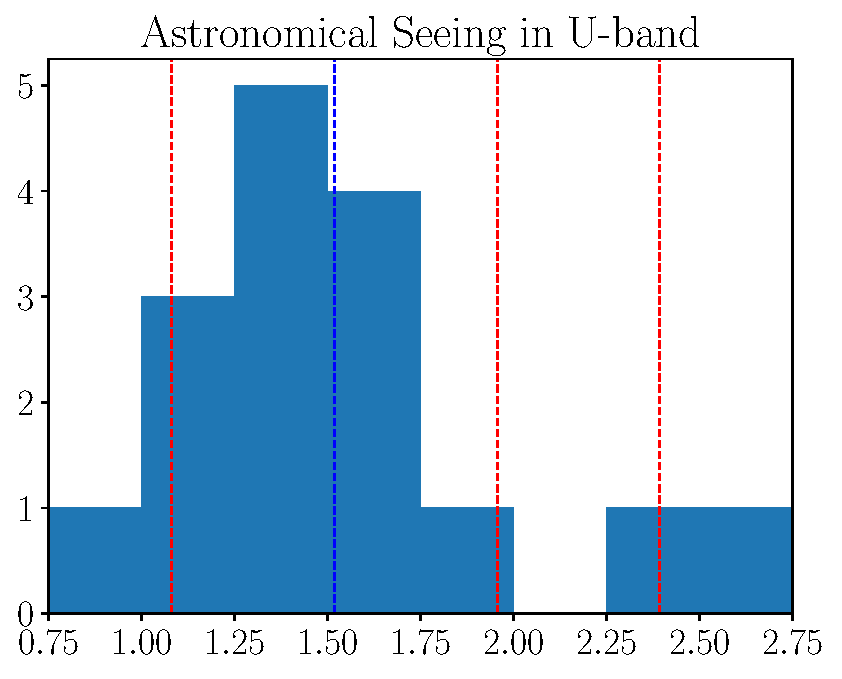
\includegraphics[width=0.32\textwidth]{seeing_hist_U_band.eps}
    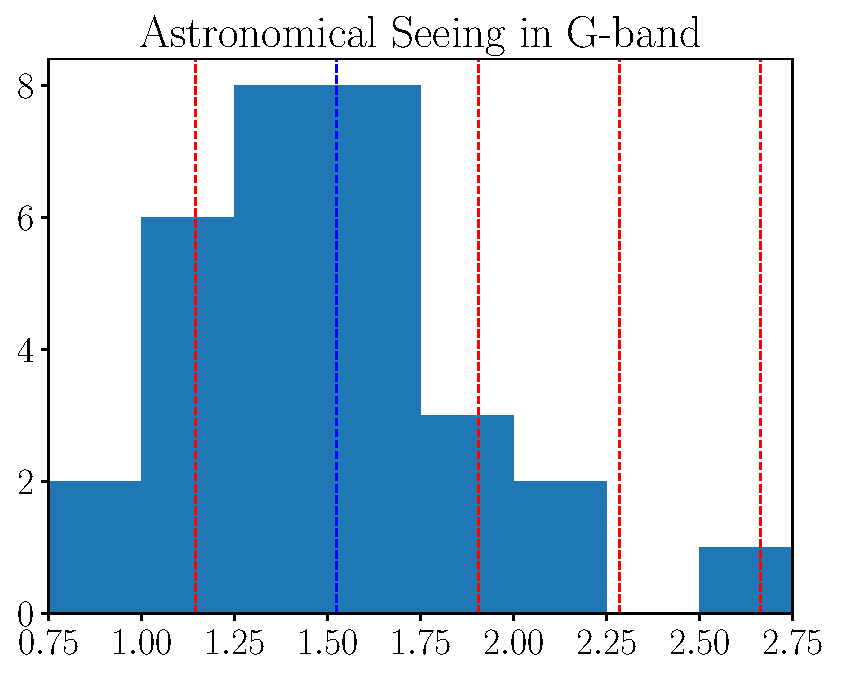
\includegraphics[width=0.32\textwidth]{seeing_hist_G_band.eps}
    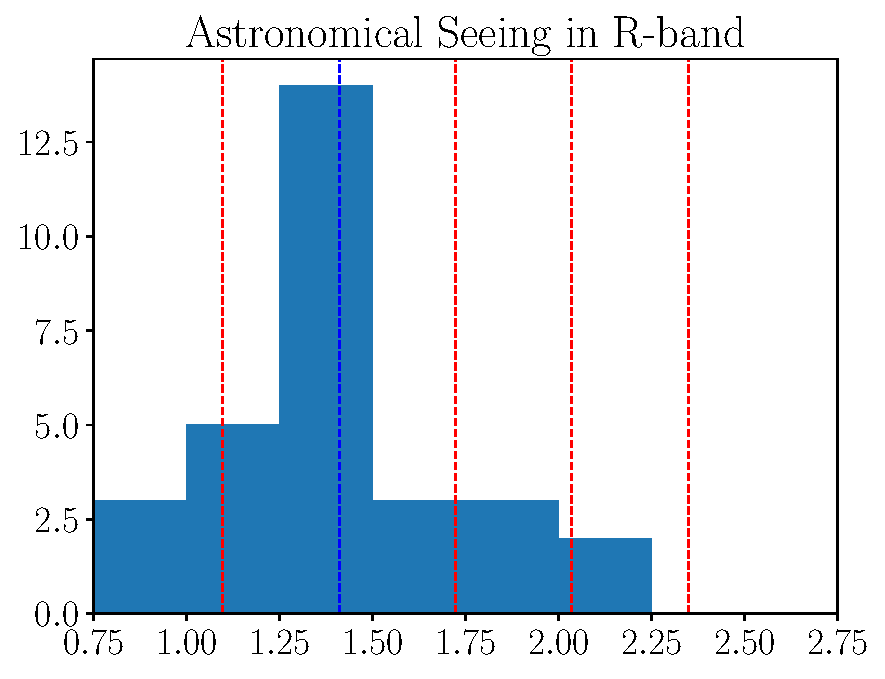
\includegraphics[width=0.32\textwidth]{seeing_hist_R_band.eps}
    \caption{Astronomical seeing of the LT data in Johnson UGR bands.}
    \label{fig:seeing}
\end{figure}

There are several technical problems associated with the Liverpool Telescope
(LT) data. In many frames, astronomical seeing is very poor. All frames,
particularly in the U-band, are littered with hot pixels or cosmic rays
detections.

A single image of J094511 in the U-band has a seeing of $r_0=999.0''$, which is
likely an error. For this reason, the image has been thrown out and its seeing
parameter excluded from the calculation of the mean and standard deviation of
the seeing data.

\subsection{S/N Ratio and Astronomical Seeing}
\section{Centroiding on J094511}
\subsection{Initial Guess: Max-Value Centroiding}
\subsection{Initial Guess: WCS Centroiding}

\begin{figure}[H]
    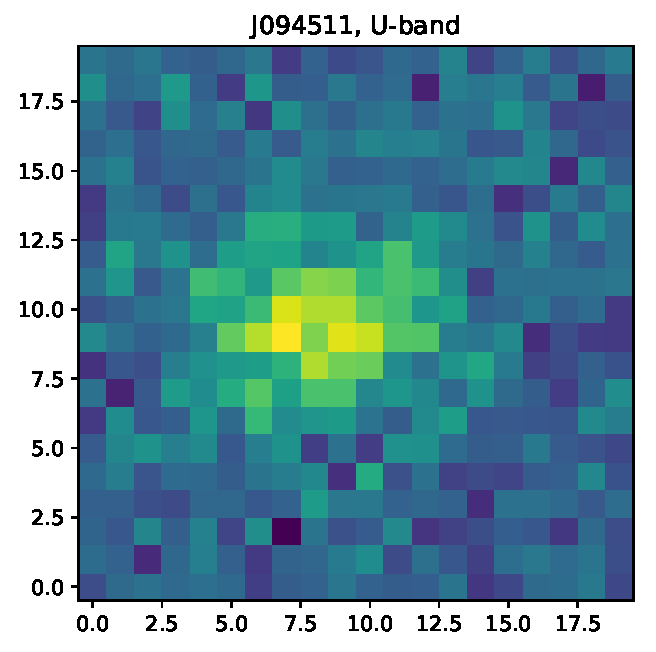
\includegraphics[width=0.32\textwidth]{wcs_centroid_U_stack.eps}
    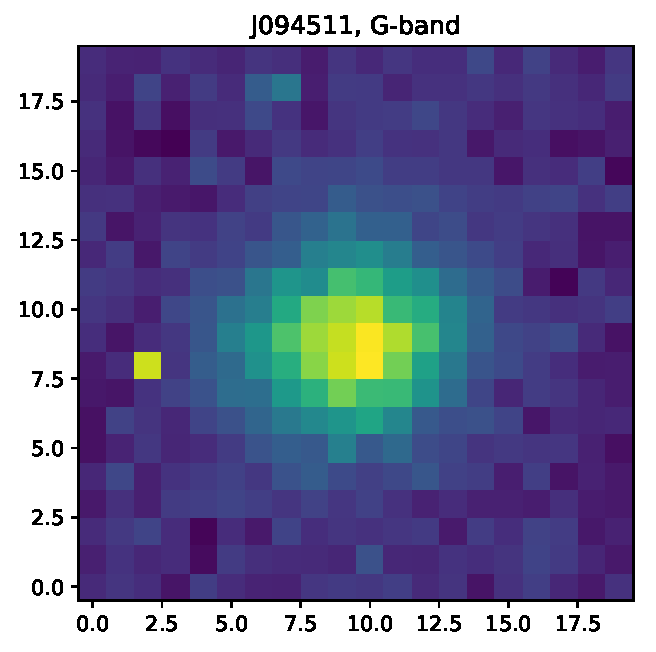
\includegraphics[width=0.32\textwidth]{wcs_centroid_G_stack.eps}
    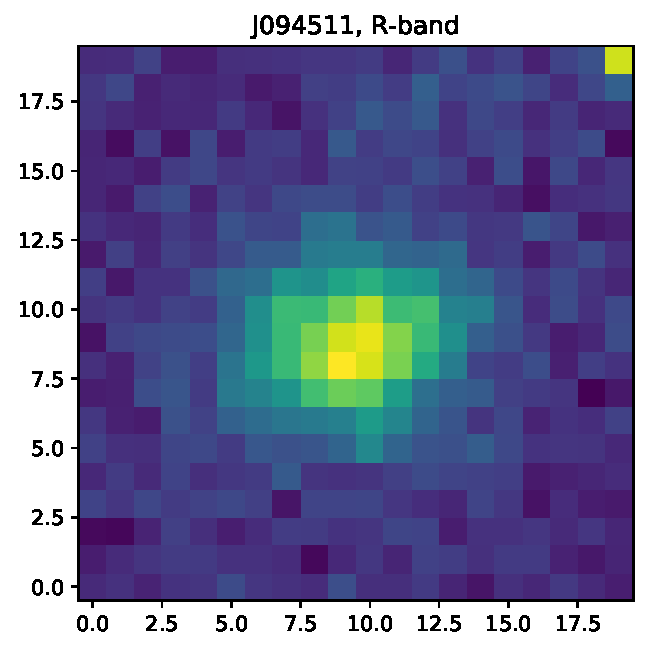
\includegraphics[width=0.32\textwidth]{wcs_centroid_R_stack.eps}
    \caption{Image stack of J094511 in the Johnson UGR bands.}
    \label{fig:wcs_centroids}
\end{figure}

% \cite{lang_2010}
% \cite{greisen_2002}
% \cite{calabretta_2002}
\subsection{Refinement: Two Dimensional Weighted Mean}
\subsection{Refinement: Gaussian Fitted Centroiding}

In two dimensions, the power to which $e$ is raised in the Gaussian function is
any negative-definite quadratic form.  Consequently, the level sets of the
Gaussian will always be ellipses. A particular example of a two-dimensional
Gaussian function is:

\begin{equation}
    f(x,y) = A \exp\left(- \left(\frac{(x-x_0)^2}{2\sigma_x^2} + \frac{(y-y_0)^2}{2\sigma_y^2} \right)\right)
\end{equation}

\noindent Here, the coefficient $A$ is the amplitude, $(x_0, y_0)$ is the center and
$\sigma_x$, $\sigma_y$ are the $x$ and $y$ spreads of the blob. In general, a
two-dimensional elliptical Gaussian function is expressed as:

\begin{equation}
    f(x,y) = A \exp\left(- \left(a(x - x_0)^2 + 2b(x-x_0)(y-y_0) + c(y-y_0)^2 \right)\right)
\end{equation}

\noindent Where the matrix:

\begin{equation}
    \begin{bmatrix} a & b \\ b & c \end{bmatrix}
\end{equation}

\noindent Is positive-definite. For the general form of the equation the
coefficient $A$ is the height of the peak and $(x_0, y_0)$ is the center of the
blob. If we set:

\begin{align}
a & = \frac{\cos^2\theta}{2\sigma_x^2} + \frac{\sin^2\theta}{2\sigma_y^2} \\
b & = -\frac{\sin2\theta}{4\sigma_x^2} + \frac{\sin2\theta}{4\sigma_y^2} \\
c & = \frac{\sin^2\theta}{2\sigma_x^2} + \frac{\cos^2\theta}{2\sigma_y^2}
\end{align}

then we rotate the blob by a clockwise angle $\theta$ (for counterclockwise
rotation invert the signs in the $b$ coefficient). %<ref>{{cite web |last1=Nawri |first1=Nikolai |title=Berechnung von Kovarianzellipsen |url=http://imkbemu.physik.uni-karlsruhe.de/~eisatlas/covariance_ellipses.pdf |accessdate=14 August 2019}}</ref>

\subsection{Aperture Centroiding}
\subsection{Challenges in the U-band}
\section{Cross Sections of J094511}
\subsection{Linear and Radial Cross Sections}
\subsection{Excess Luminosity in the Wings}
\subsection{Point Spread Function Subtraction}
\section{Analysis}
\section{Conclusion}




\section*{Appendix A: Alignment Algorithm}

\end{document}
